% -*- latex -*-

\chapter{Tutorial}
\label{chap:Tutorial}

In this chapter we outline the steps required to create a simple \IceT
application from building the \IceT source, using the created libraries,
and writing your own applications.  \IceT is solely responsible for the
image composition part of parallel rendering.  Thus, it relies on separate
systems for rendering and communication.  The two most common libraries
for these features are \index{OpenGL}\keyterm{OpenGL} and
\index{MPI}\keyterm{MPI} (the Message Passing Interface), respectively.
\IceT has support libraries for directly using these two systems and we
will use them for this tutorial.

This tutorial assumes the reader is familiar with \OpenGL or some similar
rendering system.  If this is your first experience with \OpenGL programing,
consider trying some typical serial rendering before jumping into the
parallel rendering domain.  A familiarity with \MPI is also helpful.

\section{Building \IceT}
\label{sec:Tutorial:Building_IceT}

The \IceT build process is very portable.  It is regularly compiled on
Microsoft Windows, Macintosh OS X, and a wide variety of Unix
implementations.  \IceT can be built with any \index{OpenGL}OpenGL~1.1
compliant installation.  Most modern operating systems come distributed
with \OpenGL.  For those that are not, you can usually use the
\index{Mesa~3D}\keyterm{Mesa 3D} library
(\href{www.mesa3d.org}{www.mesa3d.org}), a software implementation of
\OpenGL.  An installation of \MPI is also almost always needed, although not
strictly required.  \index{MPICH}\keyterm{MPICH}
(\href{http://www-unix.mcs.anl.gov/mpi/mpich2/}{http://www-unix.mcs.anl.gov/mpi/mpich2/})
is a free and widely portable implementation of \MPI.

% TODO: add OpenMPI.

\IceT uses \index{CMake}\keyterm{CMake} to build across so many different
platforms.  As such, you will have to download the CMake build tools from
\href{www.cmake.org}{www.cmake.org} and install.  Then, create a build
directory and run the CMake program (from the ``Start'' menu on Windows or
ccmake on Unix and Mac OS X).  CMake will determine the parameters of your
system and do its best to find libraries on which \IceT depends.  The CMake
program, shown in Figure~\ref{fig:Tutorial:ccmake} will also provide a GUI
to allow you to easily change build parameters and external libraries.
\begin{figure}
  \centering
  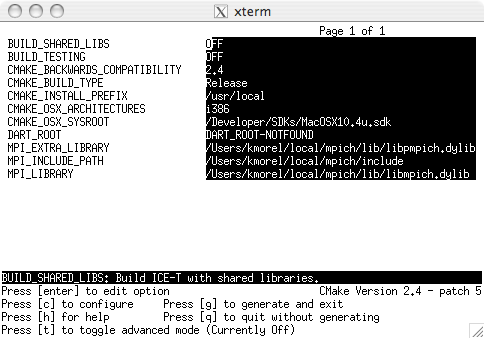
\includegraphics[height=1.5in]{images/ccmakeUnix}
  \qquad
  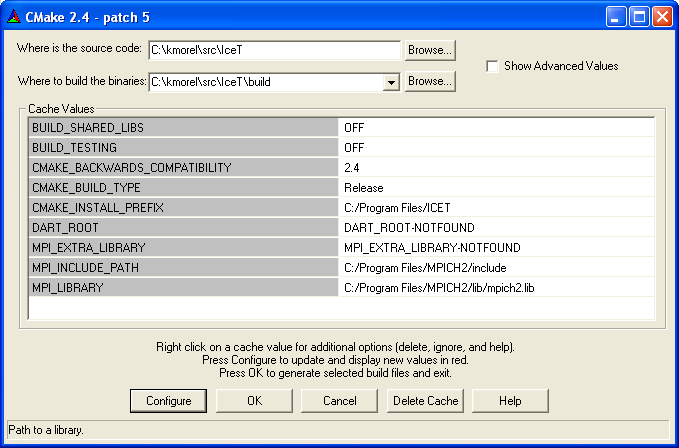
\includegraphics[height=1.5in]{images/ccmakeWindows}
  \caption[CMake user interface.]{The CMake user interface.  The Unix
    version is on the left whereas the Microsoft Windows version is on the
    right.}
  \label{fig:Tutorial:ccmake}
\end{figure}

CMake will generate a set of build files for the local system.  The type of
files depends on the type of machine you are using and the compile system
you have chosen to use.  On Unix machines, make files are the most common.
On Windows, you usually generate MSVC project files or nmake files.  On Mac
OS X, either make files or Xcode project files are commonly generated based
on user selection.  You then use the native build system to build and,
optionally, install \IceT.

\section{Linking to \IceT Libraries}
\label{sec:Tutorial:Linking_to_IceT_Libraries}

\IceT comes with four libraries: \index{IceT (library)}\keyterm{IceT},
\index{IceTStrategies~(library)}\keyterm{IceTStrategies},
\index{IceTGL~(library)}\keyterm{IceTGL}, and
\index{IceTMPI~(library)}\keyterm{IceTMPI}.  The actual filenames of these
libraries varies depending on the filesystem and build type.  For example,
on most Unix systems, a static build results in filenames of
\index{libIceT.a}libIceT.a and the like whereas shared libraries are
\index{libIceT.so}libIceT.so.  Windows has libraries with names like
\index{IceT.lib}IceT.lib as well as \index{IceT.dll}IceT.dll if building
shared libraries.  However, the difference in these filenames usually
hidden by the build system, especially if you use a portable build system
like \index{CMake}CMake.

You are, of course, free to use whatever build system you like, whether it
be system specific or cross platform.  Using \IceT is simply a matter of
finding the header and library files.  However, because \IceT is built with
\index{CMake}CMake, it comes with some extra facilities for helping other
CMake builds find it.  This section will give you the bare minimum you need
to set up CMake to build an application using \IceT.  Readers interested in
learning more about CMake should pick up a copy of \emph{Mastering CMake}
by Ken Martin and Bill Hoffman.

You define a build system with CMake by creating a
\index{CMakeLists.txt}\keyterm{CMakeLists.txt} file.  The CMakeLists.txt
file is basically a simple script that gives commands to CMake to tell it
how to build your project.  Most CMakeLists.txt files start with the
\textC{PROJECT} command, which associates a name with your project and
optionally specifies a language.
\begin{code}
PROJECT(IceT_Tutorial)
\end{code}

To use \IceT from within your CMake project, run the
\index{FIND\_PACKAGE}\textC{FIND\_PACKAGE} command.  This command instructs
CMake to find the \index{IceTConfig.cmake}IceTConfig.cmake file, which is
written to \IceT's build or install directory and contains all the
necessary build settings.
\begin{code}
FIND_PACKAGE(IceT REQUIRED)

INCLUDE_DIRECTORIES(${ICET_INCLUDE_DIRECTORIES})
\end{code}
%$

Assuming that CMake finds \IceT, the CMake variable
\CEnum{ICET\_INCLUDE\_DIRS} is defined and can be passed to the
\index{INCLUDE\_DIRECTORIES}\textC{INCLUDE\_DIRECTORIES} CMake command.
The variables \CEnum{ICET\_CORE\_LIBS}, \CEnum{ICET\_GL\_LIBS}, and
\CEnum{ICET\_MPI\_LIBS} are also defined and can be used with a
\index{TARGET\_LINK\_LIBRARIES}TARGET\_LINK\_LIBRARIES command to link in
the respective \IceT libraries.

Any application using \IceT will probably also be using \OpenGL and \MPI.
In addition, the example in the following section also uses
\index{GLUT}GLUT for window management.  CMake comes with modules to find
all three of these libraries, which makes it easy to include in our
project.

\begin{code}
FIND_PACKAGE(OpenGL REQUIRED)
FIND_PACKAGE(GLUT REQUIRED)
FIND_PACKAGE(MPI REQUIRED)

MARK_AS_ADVANCED(CLEAR
  MPI_INCLUDE_PATH
  MPI_LIBRARY
  MPI_EXTRA_LIBRARY
  )

INCLUDE_DIRECTORIES(
  ${OPENGL_INCLUDE_DIR}
  ${MPI_INCLUDE_PATH}
  ${GLUT_INCLUDE_DIR}
  )
\end{code}
%$

The only thing left to do is to tell CMake to build a program from a set of
sources and libraries specified with the
\index{ADD\_EXECUTABLE}\textC{ADD\_EXECUTABLE} and
\index{TARGET\_LINK\_LIBRARIES}\textC{TARGET\_LINK\_LIBRARIES} commands,
respectively.
\begin{code}
ADD_EXECUTABLE(Tutorial Tutorial.c)
TARGET_LINK_LIBRARIES(Tutorial
  ${OPENGL_LIBRARIES}
  ${GLUT_LIBRARIES}
  ${MPI_LIBRARY}
  ${MPI_EXTRA_LIBRARY}
  ${ICET_CORE_LIBS}
  ${ICET_GL_LIBS}
  ${ICET_MPI_LIBS}
  )
\end{code}
%$

\section{Creating \IceT Enabled Applications}
\label{sec:Tutorial:Creating_IceT_Enabled_Applications}

To use \IceT, include its header: \index{IceT.h}\textC{IceT.h}.  If you are
using \OpenGL for rendering, you will probably also want to use \IceT's
\OpenGL integration functions in \index{IceTGL.h}\textC{IceTGL.h}.  You will
almost always need to also include the header containing an \MPI version of
an \IceT communicator: \index{IceTMPI.h}\textC{IceTMPI.h}.  On the rare
occasion that you need to use \IceT with a communication layer other than
\MPI, you can define a custom communicator as described in
Chapter~\ref{chap:Communicators}.
\begin{code}
#include <IceT.h>
#include <IceTGL.h>
#include <IceTMPI.h>
\end{code}

Before you call any \IceT functions, you need to initialize \MPI by calling
\textC{MPI\_Init}\index{MPI\_Init}.  You will also need to create an
\index{context!\OpenGL}\keyterm{\OpenGL context}.  In other words, you need
to make the rendering window in which the \OpenGL rendering commands will
go.  The process for doing this is greatly dependent on the windowing
system and beyond the scope of this document.  It is usually easiest to use
a third party API to do this.  If you are not already using a GUI tool that
generates \OpenGL windows for you, then the \index{GLUT}\keyterm{GLUT} API
is a popular choice for simple applications.

You will then need to initialize \IceT itself.  Do this by first creating
an \IceT \index{communicator}\keyterm{communicator} from an \MPI
communicator and then using that to create an
\index{context!\IceT}\keyterm{\IceT context}.  When using \OpenGL, you also
need to initialize the OpenGL-specific code in \IceT by calling
\CFunc{icetGLInitialize}.

\index{icetCreateMPICommunicator}
\index{icetCreateContext}
\begin{code}
    comm = icetCreateMPICommunicator(MPI_COMM_WORLD);
    context = icetCreateContext(comm);
    icetGLInitialize();
\end{code}

In the proceeding code, \textC{comm} is of type
\index{IceTCommunicator}\textC{IceTCommunicator} and \textC{context} is of
type \index{IceTContext}\textC{IceTContext}.

Now that we have created and activated an \IceT communicator, as well as
initialized the \IceT \index{state}\keyterm{state}, we can start using
\IceT.  It is often useful to first query \IceT on the size of the parallel
job it is running in and what is the local process id, or
\index{rank}\keyterm{rank}.  The values are stored in variables of type
\index{IceTInt}\textC{IceTInt}.

\index{icetGetIntegerv}
\index{ICET\_RANK}
\index{ICET\_NUM\_PROCESSES}
\begin{code}
    icetGetIntegerv(ICET_RANK, &rank);
    icetGetIntegerv(ICET_NUM_PROCESSES, &num_proc);
\end{code}

Before rendering, we need to tell \IceT the layout of the tiled display
using the \CFunc{icetResetTiles} and \CFunc{icetAddTile} functions.  These
commands must be executed with the same arguments on all processes of the
parallel job.  \IceT will assume that you setup the same display layout
everywhere.

If you are not actually driving a tiled display and instead just generating
a desktop-sized image, the following commands will correctly establish the
\IceT state (assuming \textC{WINDOW\_WIDTH} and \textC{WINDOW\_HEIGHT}
correctly reflect the desired image dimensions).

\begin{code}
    icetResetTiles();
    icetAddTile(0, 0, WINDOW_WIDTH, WINDOW_HEIGHT, 0);
\end{code}

The \CFunc{icetResetTiles} function simply tells \IceT that you are about
to define a display layout.  Each call to \CFunc{icetAddTile} defines a
tile in the display.  In the case of a single image, the
\index{single-tile~rendering}\keyterm{single-tile rendering} mode,
\CFunc{icetAddTile} is called only once.  The first two arguments to
\CFunc{icetAddTile} have no effect in this mode.  The third and fourth
arguments are the width and height of the image to create.  Usually you set
this to the width and the height of the display window, but the
\hyperref[sec:Customizing_Compositing:Image_Inflation]{Image Inflation}
section in Chapter~\ref{chap:Customizing_Compositing} describes other usage
for these parameters.  The final argument is the rank of the
\index{display~process}\keyterm{display process}.  After a rendering the
final complete image will available only on this process.  In the example
above, we have directed the image to go to process zero, often referred to
as the \index{root~process}\keyterm{root process}.

To define an actual tiled display, simply call the \CFunc{icetAddTile}
function multiple times.  When describing tiles in a display, the first two
arguments of \CFunc{icetAddTile} describe where the lower left corner of
the tile is located in respect to the overall display.  All together, the
first four arguments specify a viewport for the tile in an a single,
cohesive high resolution display (which is what we are trying to achieve
with our tiled display).  The code below defines a $2 \times 2$ tiled
display with the top two tiles displayed by processes 0 and 1 and the
bottom two tiles displayed by processes 2 and 3.
\begin{code}
    icetResetTiles();
    icetAddTile(0,           WINDOW_HEIGHT, WINDOW_WIDTH, WINDOW_HEIGHT, 0);
    icetAddTile(WINDOW_WIDTH,WINDOW_HEIGHT, WINDOW_WIDTH, WINDOW_HEIGHT, 1);
    icetAddTile(0,           0,             WINDOW_WIDTH, WINDOW_HEIGHT, 2);
    icetAddTile(WINDOW_WIDTH,0,             WINDOW_WIDTH, WINDOW_HEIGHT, 3);
\end{code}

\IceT contains several \index{strategy}\keyterm{strategies} for image
composition.  Changing the strategy modifies the algorithm \IceT uses for
parallel image compositing.  You need to tell \IceT which strategy to use
with the \CFunc{icetStrategy} function.  The code below sets \IceT to use
the \index{strategy!reduce}\keyterm{reduce strategy}, which has proven to
be an all-around good performer.
\begin{code}
    icetStrategy(ICET_STRATEGY_REDUCE);
\end{code}
Like with the display set up, all processes must set the same strategy.

\IceT is almost ready to go.  We just need to tell it some minimal
information about how to render your geometry.  First, \IceT needs to know
the spatial extent of the geometry to be drawn (in object space).  The most
natural way to do this is to use the \CFunc{icetBoundingBox} function,
which defines an axis-aligned box defined by the minimum and maximum
coordinates in each dimension.
\begin{code}
    icetBoundingBoxf(x_min, x_max, y_min, y_max, z_min, z_max);
\end{code}
The parameters can, and should be, different on each process, since each
process will have a different partition of data.  Strictly speaking,
identifying the geometry bounds is not necessary.  If they are not defined,
\IceT will assume the geometry covers the entire screen.  When rendering a
single small image, the information is of little consequence.  However,
when rendering larger images this information can dramatically improve the
performance of image composting.  Specifying the bounds can be critical on
large tile displays.

The second and final piece of information \IceT needs is a way to draw your
geometry.  \IceT achieves this through a
\index{drawing~callback}\index{callback|see{drawing~callback}}\index{rendering~callback|see{drawing~callback}}\keyterm{drawing
  callback}.

\index{icetGLDrawCallback}
\begin{code}
    icetGLDrawCallback(drawScene);
\end{code}

The drawing callback is a pointer to any function that issues \OpenGL
commands that render geometry to the active frame buffer.  The callback is
free to issue most \OpenGL commands so long as it restores all the \OpenGL
state (except, of course, frame buffer contents).  Also, the callback
function should modify neither the projection matrix nor the clear color.
Care needs to be taken if the callback modifies the model view matrix.
More details are given in the
\hyperref[sec:Basic_Usage::Drawing_Callback]{Drawing Callback} section of
Chapter~\ref{chap:Basic_Usage}.

\IceT is now ready to render.  Rendering is initiated with a call to
\CFunc{icetGLDrawFrame}.  The \CFunc{icetGLDrawFrame} must be called on all
processes.  The function will render the scene using the provided
\index{drawing~callback}drawing callback, composite the image, and place
the appropriate images in the back \OpenGL buffers of the appropriate
\index{display~process}display processes.
\begin{code}
    icetGLDrawFrame();
\end{code}

Parallel rendering is now enabled in your application.  Simply call
\CFunc{icetGLDrawFrame} every time you wish to draw a new image.  The
geometry rendered by your \index{drawing~callback} may change from frame to
frame so long as you ensure that you also update \IceT with the bounds of
your geometry if it changes.

The following code is a full example of a simple \IceT application.  Do not
be alarmed by the length.  The majority of the code is spent in setting up
the supporting libraries (\OpenGL, \index{GLUT}GLUT, and \MPI) and in
comments.

\codeinput{examples/Tutorial.c}
